\chapter{\acrfull{dospu}}

Según \cite{CSOrd17}, la misión de \acrshort{dospu} consiste en:

\begin{displayquote}
Entender en la organización administrativa de la Obra Social y en todos los aspectos contables, financieros y de acción social a cargo de la DOSPU.

Entender en todas las actividades inherentes a la asistencia, altas y bajas del personal de la DOSPU.

Entender en los procedimientos de incorporación, registro y documentación de las y los afiliados.

Entender en todos los aspectos de financiación, manejo de valores y recursos económicos a cargo de la DOSPU.

Entender en la supervisión del sistema de asistencia médica, odontológica, química, bioquímica, farmacéutica, psicológica y demás profesionales de la salud.

Controlar la atención médica según operatoria de Auditoría definida previamente por DOSPU.

Coordinar y organizar la provisión y expendio de los productos farmacéuticos para pacientes crónicos y de alto costo.

Instrumentar y operar las políticas, normas, sistemas y procedimientos necesarios para garantizar la exactitud y seguridad en la captación y registro de las operaciones financieras, presupuestarias y de consecución de metas de DOSPU y DECOM. Llevar el registro contable, de patrimonio, realizar el control presupuestario, refrendar y supervisar la confección de los balances, estados patrimoniales.

Supervisar la asistencia médica, sanitaria integral, sistema de reciprocidad y celebraciones de convenios con prestadores.

Asegurar la prestación de todos los servicios que ofrece la Obra Social al Personal Universitario en el Complejo Universitario de Villa Mercedes.
\hfill\parencite{CSOrd17}
\end{displayquote}

Por otra parte, dado el tamaño de la dirección, esta se encuentra divivida en varias direcciones que, a su vez, son dividas en departamentos (ver \cref{fig:estructura_dospu}). En las siguientes secciones se encuentran las tareas de las que se ocupa cada una de las direcciones y los departamentos de \acrshort{dospu}.

\begin{figure}
    \centering
    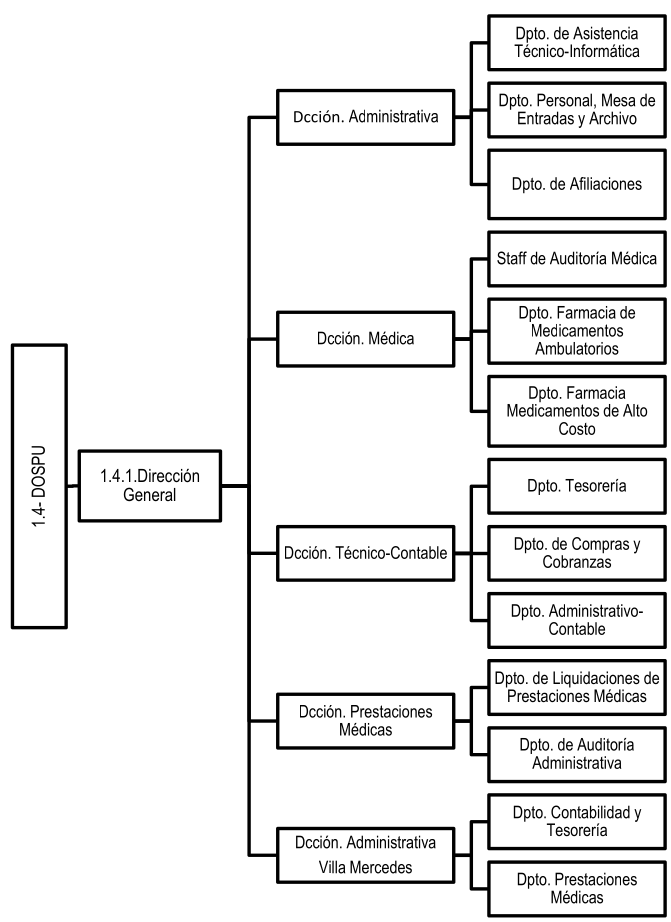
\includegraphics[width=\textwidth]{estructura_dospu.png}
    \caption{Estructura organizacional \acrshort{dospu} \cite{CSOrd17}}
    \label{fig:estructura_dospu}
\end{figure}

\section{Dirección General}
\begin{displayquote}
a) Asistir a la Presidencia en la confección de resoluciones, providencias, ordenanzas, notas, comunicaciones y sus respectivos registros.

b) Organizar la administración y servicios con acuerdo del Directorio.

c) Cumplir y hacer cumplir el Estatuto, las reglamentaciones y resoluciones de la Obra Social.

d) Someter a consideración de Presidencia y el Directorio, las contrataciones correspondientes a la prestación de servicios.

e) Colaborar en el diseño de todas las medidas que sean necesarias para la solución de problemas de afiliados que sean de competencia de la Obra Social.

f) Controlar y verificar todo lo concerniente a la contabilidad y control económico-financiero y de la prestación de los servicios.

g) Elevar mensualmente a consideración del Directorio un informe demostrativo de la situación económica-financiera de DOSPU y DECOM, juntamente con referencias estadísticas que permitan orientar la acción a seguir en base a las posibilidades económicas.

h) Ofrecer al Directorio informes demostrativos de la situación económico-financiera de DOSPU y DECOM, con referencias estadísticas que permitan orientar la acción a seguir en base a las posibilidades económicas.

i) Firmar los estados mensuales de caja, cuadros estadísticos, inventarios y balances.

j) Suscribir juntamente con Presidencia la documentación relativa a pagos y promesas de pago, como así también las contrataciones con terceros.

k) Suscribir con Presidencia la Memoria de DOSPU y DECOM.

l) Suscribir los estados mensuales de caja, cuadros estadísticos, inventarios y balances.

m) Solicitar al Directorio la aplicación de sanciones disciplinarias a los afiliados que no cumplan con las disposiciones de DOSPU y DECOM.

n) Entender en la representación de DOSPU ante otras Obras Sociales con las que se firmen convenios de Reciprocidad, a pedido de Presidencia.

o) Conservar los antecedentes y documentación de los acuerdos del Directorio.

p) Intervenir en la difusión, resolución y ejecución de todos los asuntos relativos a los intereses de la obra social.

q) Desempeñar toda otra actividad que la autoridad le encomiende, en el área de trabajo y de
acuerdo con la responsabilidad específica.
\hfill\parencite{CSOrd17}
\end{displayquote}

\section{Dirección Administrativa}
\begin{displayquote}
a) Asistir a la Presidencia en la confección de resoluciones, providencias, ordenanzas, notas, comunicaciones y sus respectivos registros.

b) Administrar los subsidios que se reglamenten y el panteón de la DOSPU.

c) Entender en todo lo relativo a ejecución, registro, identificación y manejo interno de la documentación que ingresa a la DOSPU y DECOM.

d) Organizar y controlar las Actividades/Tareas de vigilancia y limpieza.

f) Desempeñar toda otra actividad que la autoridad le encomiende, en el área de trabajo y de acuerdo con la responsabilidad específica.
\hfill\parencite{CSOrd17}
\end{displayquote}

\subsection{Departamento de Asistencia Técnico-Informática}
\begin{displayquote}
a) Realizar la correcta instalación física de servidores de red y dispositivos de comunicación, el software y la configuración de este, la actualización de los sistemas operativos y dispositivos de conectividad cumpliendo los requerimientos de seguridad informática establecidos para la operación, administración y comunicación de los sistemas y recursos de tecnología de la Universidad.

b) Realizar Actividades/Tareas de mantenimiento preventivo en cableados y configuración de redes, hardware y software de equipos.

c) Confeccionar un registro de todas las fallas críticas producidas en la red de equipamientos.

d) Monitorear la utilización de Internet, correo electrónico y demás tráfico de red.

e) Administrar los usuarios de la red, su seguridad, tanto en los servidores como en los dispositivos de comunicación (routers, switches, y estaciones de trabajo), y del desarrollo de procedimientos de automatización de Actividades/Tareas.

f) Controlar la asignación de privilegios a usuarios.

g) Sugerir medidas a ser implementadas para efectivizar el control de acceso y uso de Internet de los distintos usuarios.

h) Realizar la investigación y puesta en funcionamiento de nuevos clientes de software, y proveer a la capacitación de los agentes para estos fines.

i) Colaborar en la investigación de nuevas tecnologías para redes y comunicaciones, tanto de software como hardware, la confección de los borradores de pliegos de bases y condiciones y la supervisión en las prestaciones de servicios de obras ejecutadas por administración o por terceros.

j) Realizar el soporte a usuarios en el correcto manejo de los dispositivos de hardware y software.

k) Participar en la definición de normas y procedimientos de seguridad a implementar en el ambiente informático.

l) Ejercer el soporte y mantenimiento de la infraestructura de conectividad a la Internet. m) Responder por la instalación y mantenimiento de la estructura de interconexión de las sedes de DOSPU y DECOM.

n) Establecer y fomentar estándares de compras de equipamiento informático.

o) Mantenimiento de la infraestructura eléctrica y de soporte para los servidores

p) Realizar las Actividades/Tareas de diseño, codificación e implementación de los sistemas que se desarrollen en el área.

q) Supervisar la prestación de servicio u obra ejecutada por administración o por terceros en los desarrollos de sistemas.

r) Evaluar la necesidad de nuevos sistemas y sugerir prioridades de desarrollo.

s) Entender en la determinación de los controles y seguridad informática interna.

t) Desempeñar toda otra tarea que la autoridad le encomiende, en el área de trabajo y de acuerdo con la responsabilidad específica.
\hfill\parencite{CSOrd17}
\end{displayquote}

\section{Dirección Médica}
\begin{displayquote}
a) Colaborar con la Presidencia de la DOSPU en la presentación anual del Plan de proyectos a concretar en el área.

b) Efectuar Actividades/Tareas de supervisión médica y odontológica.

c) Supervisar a los Auditores Médicos y Odontológicos.

d) Supervisar a la Farmacia en los aspectos médicos de las compras que se efectúen, formar parte de la Comisión de Vademécum y establecer pautas conjuntas de trabajo.

e) Supervisar a Enfermería.

f) Supervisar la tarea de los profesionales en los Consultorios Internos confeccionando el Organigrama y distribución de los Consultorios e incorporación de profesionales.

g) Intervenir como Asesor en la celebración de convenios con entidades de profesionales de la salud.

h) Participar como Jurado en la selección de profesionales para el servicio interno de la obra social.

i) Ejercer el control y supervisión de las Actividades/Tareas de las Áreas pertenecientes a la Dirección.

j) Organizar la implementación de los planes y programas de prevención.

k) Coordinar la prestación de los servicios en las diferentes sedes.

l) Gestionar el funcionamiento de los servicios propios.

m) Organizar y coordinar el servicio de atención personalizada de los beneficiarios.

n) Recepcionar, tramitar y coordinar la entrega de recetarios de prescripción de medicamentos a los beneficiarios, por el tratamiento de afecciones crónicas y de largo tratamiento.

o) Mantener actualizado el archivo de historias clínicas.

p) Organizar las Actividades/Tareas auxiliares de la medicina y asistencia en los consultorios de prestaciones médicas, odontológicas, quinesiológicas, etc.

q) Desempeñar toda otra actividad que la autoridad le encomiende, en el área de trabajo y de acuerdo con la responsabilidad específica.
\hfill\parencite{CSOrd17}
\end{displayquote}

\subsection{Staff de Auditoría Interna}
\begin{displayquote}
a) Intervenir en la autorización y diligenciamiento de las prestaciones solicitadas por los afiliados.

b) Dar cumplimiento a las normas de calidad de atención médica.

c) Actualización de normas según la evolución de la ciencia médica y leyes nacionales vigentes.
d) Autorizar el Ingreso de Afiliados Adherentes.

e) Comprobar la capacidad estructural de los prestadores, con relación a lo ofrecido.

f) Evaluación de los servicios de internación mediante Auditoria de Terreno. Juntamente de manera inmediatamente elevará informe a Dirección Médica.

g) Auditar, junto a la Dirección de Prestaciones Médicas, la facturación presentada por los prestadores, a los fines de cotejar los valores contractuales, codificación, servicios prestados, calidad de atención médica, etc.

h) Confeccionar indicadores a los fines de detectar desvíos en los servicios prestados.

i) Participar en la confección de convenios con prestadores externos e internos.

j) Análisis de propuestas arancelarias.

k) Control de prestadores asistenciales.

l) Evaluación de autorización de prácticas de Alta Complejidad.

m) Desempeñar toda otra actividad que la autoridad le encomiende, en el área de trabajo y de acuerdo con la responsabilidad específica.
\hfill\parencite{CSOrd17}
\end{displayquote}

\subsection{Departamento de Medicamentos Ambulatorios}
\begin{displayquote}
a) Supervisar el registro de ingreso, archivo y circulación de la documentación que ingrese al área.

b) Elevar informe anual de actividades de la dependencia a su cargo.

c) Mantener registro actualizado de las existencias y necesidades de la renovación del stock de medicamentos ambulatorios.

d) Gestionar las compras de medicamentos ambulatorios, registro y métodos de conservación de todos los medicamentos.

e) Gestionar los registros de medicamentos y métodos de conservación.

f) Realizar controles permanentes del stock y de los registros de adquisición y venta de los medicamentos.

g) Desempeñar toda otra actividad que la autoridad le encomiende, en el área de trabajo y de acuerdo con la responsabilidad específica.
\hfill\parencite{CSOrd17}
\end{displayquote}

\subsection{Departamento Farmacia Medicamentos de Alto Costo}
\begin{displayquote}
a) Supervisar el registro de ingreso, archivo y circulación de la documentación que ingrese al área.

b) Elevar informe anual de actividades de la dependencia a su cargo.

c) Mantener registro actualizado de las existencias y necesidades de la renovación del stock de medicamentos para pacientes crónicos y alto costo.

d) Asistir técnicamente al “Departamento de Servicios Generales, Compras y Contrataciones” en los procesos de compra de los medicamentos de alto costo, diabetes y de los que el Directorio determine por resolución.

e) Gestionar los registros de medicamentos y métodos de conservación.

f) Realizar controles permanentes del stock y de los registros de adquisición y venta de los medicamentos.

g) Desempeñar toda otra actividad que la autoridad le encomiende, en el área de trabajo y de acuerdo con la responsabilidad específica.
\hfill\parencite{CSOrd17}
\end{displayquote}

\section{Dirección Técnico-Contable}
\begin{displayquote}
a) Colaborar en la elaboración de las resoluciones y/o documentos propios de su sector.

b) Entender y supervisar todos los aspectos de financiación, manejo de valores y recursos económicos a cargo de la DOSPU.

c) Responder por el registro y depósito bancario en las cuentas bancarias correspondientes de la totalidad de los ingresos.

d) Supervisar y Refrendar la confección de los balances.

e) Dar cuenta demostrativa de los recursos y gastos y del estado económico-financiero de la Obra Social con referencias estadísticas.

f) Responder por el movimiento patrimonial de la Obra Social.

g) Proponer al Presidente/a de la Obra Social todos los cambios, modificaciones, que considere oportunos para el mejor desenvolvimiento de las Actividades/Tareas y servicios del Departamento.

h) Supervisar el sistema de Afiliaciones y el movimiento de Personal y mesa de entradas.

i) Realizar el registro de las operaciones contables de la obra social.

j) Suscribir a Presidencia el Balance Anual, cuenta de ingreso y egreso anuales.

k) Elevar mensualmente a consideración del Directorio un informe demostrativo de la situación económica-financiera de DOSPU, juntamente con referencias estadísticas que permitan orientar la acción a seguir en base a las posibilidades económicas.

l) Dar cuenta demostrativa de los recursos y gastos y del estado económico-financiero de DOSPU y DECOM con referencias estadísticas.

m) Responder por el registro y depósito bancario en las cuentas bancarias correspondientes de la totalidad de los ingresos y por el movimiento patrimonial de DOSPU y DECOM.

n) Elaborar informes sobre el movimiento patrimonial de la Obra Social. o) Desempeñar toda otra actividad que la autoridad le encomiende, en el área de trabajo y de acuerdo con la responsabilidad específica.
\hfill\parencite{CSOrd17}
\end{displayquote}

\subsection{Departamento Tesorería}
\begin{displayquote}
a) Supervisar el registro de ingreso, archivo y circulación de los expedientes, actuaciones y toda otra documentación que ingrese al área.

b) Colaborar en la elaboración de resoluciones y/o documentos propios de su sector.

c) Recibir recaudaciones diarias, controlarlas y depositarlas.

d) Efectuar los pagos a proveedores, agentes y afiliados.

e) Controlar los ingresos y egresos de la Delegación Villa Mercedes.

f) Realizar el control presupuestario y las rendiciones de cuentas de recursos.

g) Verificar las liquidaciones de aporte a cargo de los afiliados y contribución de todas las dependencias universitarias y controlar sus ingresos.

h) Desempeñar toda otra actividad que la autoridad le encomiende, en el área de trabajo y de acuerdo con la responsabilidad específica.
\hfill\parencite{CSOrd17}
\end{displayquote}

\subsection{Departamento de Compras y Cobranzas}
\begin{displayquote}
a) Entender en las adquisiciones de artículos y materiales para DOSPU y DECOM.

b) Gestionar junto con los Departamentos de Farmacia en la compra de medicamentos de alto costo y diabetes y de todos los medicamentos que el directorio determine por resolución, El Departamento de Farmacia realizará el asesoramiento técnico.

c) Controlar las adquisiciones o ventas que realicen DOSPU y De.COM.

d) Dar curso a los expedientes para la provisión anual de determinados servicios.

e) Controlar la documentación recibida y verificar el cumplimiento de los requisitos exigidos por la normativa vigente.

f) Redactar Contratos, controlar su vigencia, realizar la afectación presupuestaria de los mismos y elevar esta información a las Autoridades.

g) Conservar los contratos y legajos del personal médicos y personal administrativo que haya sido contratado.

h) Colaborar en la presentación de licitaciones, concursos de precios y compras directas.

i) Intervenir en las Comisión Evaluadora y mantener un registro actualizado de compras.

j) Intervenir y coordinar los servicios de seguridad, ambiente, mantenimiento y servicios generales.

k) Supervisar los servicios generales relativos a limpieza y conservación de bienes de DOSPU y DECOM

l) Gestionar las compras de medicamentos de alto costo y diabetes y de todos los medicamentos que el directorio determine por resolución, El Departamento de Farmacia realizara el asesoramiento técnico.

m) Llevar la cartera de cobros y pagos.

n) Desempeñar toda otra actividad que la autoridad le encomiende, en el área de trabajo y de acuerdo con la responsabilidad específica.
\hfill\parencite{CSOrd17}
\end{displayquote}

\subsection{Departamento Administrativo-Contable}
\begin{displayquote}
a) Atención de proveedores, afiliados y entidades financieras.

b) Cargo oportuno de las facturas en el sistema.

c) Control de pagos, tanto a proveedores, como parafiscales e impuestos y tributos. Control de los egresos.

d) Control de facturas y cumplimiento del marco legal vigente, así como también verificar el registro y control de notas de crédito.

e) Realización de notas de débito, conciliaciones bancarias, declaraciones y pagos fiscales.

f) Elaborar libros contables, informes de contabilidad, proyección financiera y flujo de caja, y proyección de los estados financieros.

g) Colaborar en operaciones comerciales (buscar diferentes opciones presupuestarias para cualquier compra o gasto).

h) Colaborar en el manejo del inventario.

i) Desempeñar toda otra actividad que la autoridad le encomiende, en el área de trabajo y de acuerdo con la responsabilidad específica.
\hfill\parencite{CSOrd17}
\end{displayquote}

\section{Dirección de Prestaciones Médicas}
\begin{displayquote}
a) Colaborar en la elaboración de documentos propios del sector.

b) Controlar y constatar las prestaciones y su facturación.

c) Emitir órdenes de pago y registrar los trámites del sistema de reciprocidad.

d) Organizar las Actividades/Tareas auxiliares de los trámites dentro del sistema de reciprocidad.

e) Proponer convenios entre prestadores a los fines de establecer cobertura de las diferentes prácticas.

f) Desempeñar toda otra actividad que la autoridad le encomiende, en el área de trabajo y de acuerdo con la responsabilidad específica.

g) Emitir informes de reciprocidades a pagar a la Dirección Contable y registrar los trámites en el sistema.
\hfill\parencite{CSOrd17}
\end{displayquote}

\subsection{Departamento de Liquidaciones de Prestaciones Médicas}
\begin{displayquote}
a) Facturación de honorarios médicos, anestesistas, cirujanos, bioquímicos, etc.

b) Informe de deuda por parte de los afiliados, prestaciones médicas.

c) Desempeñar toda otra actividad que la autoridad le encomiende, en el área de trabajo y de acuerdo con la responsabilidad específica.
\hfill\parencite{CSOrd17}
\end{displayquote}

\subsection{Departamento de Auditoría Administrativa}
\begin{displayquote}
a) Trabajar de manera conjunta con el Área de Auditoría Médica.

b) Registro de facturación de honorarios y gastos en internación.

c) Control de cruces de facturaciones de internaciones y prácticas ambulatorias.

d) Auditoría de medicación anestésica.

e) Confeccionar expedientes para la solicitud de reintegros frente a otros organismos.

f) Comprobación de valores de prestadores.

g) Comparación de valores entre prestadores.

h) Tramitar ante el Sistema Nacional de Información de Procuración y Trasplante de la República Argentina (SINTRA) toda acción que sea necesaria ante este organismo, o en el futuro el que lo supliere.

i) Desempeñar toda otra actividad que la autoridad le encomiende, en el área de trabajo y de acuerdo con la responsabilidad específica.

j) Confeccionar solicitud y liquidación de reintegros a los afiliados.

k) Realizar las Retenciones Impositivas a cada prestador y proceder a la carga al sistema de AFIP.
\hfill\parencite{CSOrd17}
\end{displayquote}

\subsection{Dirección Administrativa de Villa Mercedes}
\begin{displayquote}
a) Controlar las prestaciones y elevarlas a la Dirección de Prestaciones Médicas de San Luis, para su control y posterior pago.

b) Receptar y dar trámite a las directivas emanadas de la Sede Central.

c) Elaborar periódicamente los informes administrativos-contables y Balances y elevarlos a la Sede Central.

d) Elevar a Presidencia y Directorio el informe mensual de actividades de las dependencias a su cargo.

e) Representar al Presidente en las ocasiones que lo indica la Carta Orgánica.

f) Colaborar con la Dirección General Administrativa en la presentación de informes ante Presidencia y Directorio.

g) Desempeñar toda otra actividad que la autoridad le encomiende, en el área de trabajo y de acuerdo con la responsabilidad específica.
\hfill\parencite{CSOrd17}
\end{displayquote}
